\chapter{Mengenal Kecerdasan Buatan dan Scikit-Learn}

\section{Teori}
Praktek teori penunjang yang dikerjakan :
\begin{enumerate}
\item Sejarah Perkembangan dan Definisi \textit{Artifical Intelligence}. Artifical Intelligence atau biasa juga disebut sebagai kecerdasan buatan ini merupakan suatu ilmu pada bidang komputer yang mana dapat membuat suatu sistem yang cerdas untuk menyelesaikan suatu permasalahan.\\
Pada tahun 1956 istilah dari \textit{Artifical Intelligence} pertama kali diciptakan.Pada awal-awal munculnya kecerdasan buatan ini mengalami banyak kesuksesan, yang mana diawali dengan kesuksesan Newell dan Simon dengan sebuah program yang disebut dengan \textit{General Problem Solver}, program ini dirancang untuk menyelesaikan masalah secara manusiawi. Kemudian pada tahun 1960-an Departement Pertahanan Amerika Serikat juga ingin mengembangkan dan melatih komputer agar memiliki penalaran seperti manusia secara mendasar. Setelah itu tahun 1970-an, proyek DARPA(\textit{Defence Advanced Research Project Agency})berhasil menyelesaikan studi kasus tentang pemetaan jalan. Selanjutnya awal abad ke 21 atau lebih tepatnya pada tahun 2003, DARPA juga berhasil menciptakan asisten pribadi cerdas.Sejak itulah kecerdesasan buatan mengalami perkembangan hingga saat ini menjadi program yang sangat kompleks dengan menerapkan algoritma dan \textit{deep learning}. Oleh karena itu kecerdasan buatan mampu memberikan solusi yang kompleks untuk berbagai macam permasalahan dengan inovasi yang bervariatif.

\item Definisi supervised learning, klasifikasi, regresi dan unsupervised learning. Data set, training set dan testing set
\begin{itemize}
    \item Supervised Learning dan Unsupervised Learning
    \par
    \textit{Supervised learning} merupakan pembelajaran yang ada supervisornya maksudnya yaitu adanya tag dari data yang ditambahkan dalam mechine learning tersebut, guna untuk memprediksi suatu pola yang mana pola tersebut sudah ada contoh datanya, jadi pola tersebut merupakan hasil dari data yang sudah lengkap tadi.Sedangkan \textit{Unsupervised Learning} yaitu tidak menggunakan label dalam memprediksi targetnya melainkan dengan melihat kesamaan dari atribut yang dimiliki. Jika memiliki kesamaan dari atribut atau sifat data yang diextrak maka akan dimasukkan kedalam satu kelompok(\textit{clustering}). Sehingga dapat menimbulkan banyak kelompok.
    \item Klasifikasi dan Regresi
    \par
    Klasifikasi merupakan suatu teknik mengklasifikasikan atau menggelompokkan beberapa item item yang belum ada berlabel kedalam sebuah kelas distrit. Sedangkan Regresi merupakan suatu teknik analisis untuk mendefinisikan suatu relasi diantara dua variabel atau lebih, guna menemukan suatu fungsi model data dengan meminimalkan error atau selisih nilai prediksi dengan nilai sebenarnya.
    \item Data set, Training set dan Testing set
    \par
    Data set merupakan suatu objek yang akan mempresentasikan sebuah data dengan relasinya di memory.Kemudian Training set yaitu merupakan bagian dari data set yang bertujuan membuat suatu algoritma sesuai tujuan yang diinginkan sedangkan Testing set yaitu bagian dari data set yang bertujuan untuk melihat keakuratan dari data yang di tes.
\end{itemize}
\end{enumerate}

\section{Instalasi}
\begin{enumerate}
\item Melakukan installasi pada anaconda pormt dengan perintah " pip install -U scikit-learn".
    \begin{figure}[!htbp]
    \centering
    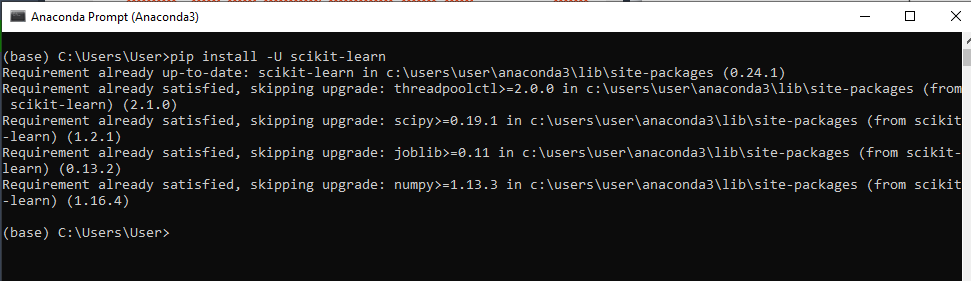
\includegraphics[scale=0.4]{figures/langkah1.PNG}
    \end{figure}
    \newpage
    \item Setelah itu masuk ke link website yang telah diberikan yaitu "https://scikit-learn.org/stable/tutorial/basic/tutorial.html".
    \begin{lstlisting}[language=Python]
from sklearn.linear_model import LogisticRegression
from sklearn import set_config


lr = LogisticRegression(penalty='l1')
print('Default representation:')
print(lr)
# LogisticRegression(C=1.0, class_weight=None, dual=False, fit_intercept=True,
#                    intercept_scaling=1, l1_ratio=None, max_iter=100,
#                    multi_class='auto', n_jobs=None, penalty='l1',
#                    random_state=None, solver='warn', tol=0.0001, verbose=0,
#                    warm_start=False)

set_config(print_changed_only=True)
print('\nWith changed_only option:')
print(lr)
# LogisticRegression(penalty='l1')
\end{lstlisting}
\item Mencoba Loading example dataset
 \begin{lstlisting}[language=Python]
from sklearn import datasets #mengimport class dataset dari scikit learn library
iris = datasets.load_iris() #memuat dan memasukkan dataset iris ke variabel bernama iris
digits = datasets.load_digits() #membuat dan memasukkan dataset digits ke variabel digits

print(digits.data) #memberikan akses ke fitur yang dapat digunakan untuk mengklasifikasikan  sampel digit dan menampilkan diconsole

digits.target #memberikan informasi tentang data yang berhubungan atau juga dapat dijadikan sebagai label

digits.images[0] #Data selalu berupa array 2D, shape (n.samples, n.features), meskipun data aslinya mungkin memiliki bentuk yang berbeda.
\end{lstlisting}
\item Mencoba Learning and predicting
\begin{lstlisting}[language=Python]
from sklearn import svm #perintah untuk mengimport class svm dari package sklearn

digits = datasets.load_digits()    #memasukkan dan memuat dataset digits ke variabel digits

clf = svm.SVC(gamma=0.001, C=100.) #elf sebagai estimator/parameter, svm.SVC sebagai class, gamma sebagai parameter untuk menerapkan nilai secara manual

clf.fit(digits.data[:-1], digits.target[:-1]) #elf sebagai estimator/parameter, fit sebagai metode, digits.data sebagai item,[:-1] sebagai syntax python dan menampilkan outputnya


print(clf.predict(digits.data[-1:])) #predict sebagai metode lainnya, digit.data sebagai item menampilkan outputnya
\end{lstlisting}
\item Mencoba Model Persistence
\begin{lstlisting}[language=Python]
from sklearn import svm #mengimport class svm dari scikit learn library
from sklearn import datasets #mengimport class dataset dari scikit learn library
 
clf = svm.SVC(gamma=0.001, C=100.) #memanggil class SVC dan menset argument constructor SVC serta ditampung di variabel clf
X, y= datasets.load_iris(return_X_y=True) #meload datasets iris dan ditampung di variabel x untuk data sedangkan y untuk target

clf.fit(X, y) #memanggil method fit untuk melakukan training data dengan argumen data dan target dari database iris 

import pickle #mengimport pickle (agar dapat terbaca)
s = pickle.dumps(clf) #memanggil method dumps dengan argumen clf dan ditampung pada valiabel s
clf2 = pickle.loads(s) #memanggil method loads dengan argumen s dan ditampung di variabel clf2
clf2.predict(X[0:1]) #menampilkan hasil dari method predict dengan argumen data variabel x 

from joblib import dump, load #mengimport dump dan load dari library joblib
dump(clf, '1184086.joblib') #memanggil method dumps dengan argumen clf dari nama file joblib
clf3 = load('1184086.joblib') #memanggil method load dengan argumen nama file joblibnya
print(clf3.predict(X[0:1])) #menampilkan hasil dari method predict dengan argumen data variabel
\end{lstlisting}
\item Mencoba Conventions
\begin{lstlisting}[language=Python]
#Type casting
import numpy as np
from sklearn import random_projection

rng = np.random.RandomState(0)
X = rng.rand(10, 2000)
X = np.array(X, dtype='float32')
print(X.dtype)


transformer = random_projection.GaussianRandomProjection()
X_new = transformer.fit_transform(X)
print(X_new.dtype)

from sklearn import datasets
from sklearn.svm import SVC
iris = datasets.load_iris()
clf = SVC(gamma=0.001, C=100.)
clf.fit(iris.data, iris.target)
print(list(clf.predict(iris.data[:3])))
clf.fit(iris.data, iris.target_names[iris.target])
print(list(clf.predict(iris.data[:3])))

#refitting and updating parameters
import numpy as np
from sklearn.datasets import load_iris
from sklearn.svm import SVC
X, y = load_iris(return_X_y=True)
clf = SVC(gamma=0.001, C=100.)
clf.set_params(kernel='linear').fit(X, y)
clf.set_params(kernel='rbf').fit(X, y)
print(clf.predict(X[:5]))

#multiclass vs multilabel fitting
from sklearn.svm import SVC
from sklearn.multiclass import OneVsRestClassifier
from sklearn.preprocessing import LabelBinarizer

X = [[1, 2], [2, 4], [4, 5], [3, 2], [3, 1]]
y = [0, 0, 1, 1, 2]

classif = OneVsRestClassifier(estimator=SVC(random_state=0, gamma=0.001, C=100.))
print(classif.fit(X, y).predict(X))
y = LabelBinarizer().fit_transform(y)
print(classif.fit(X, y).predict(X))

from sklearn.preprocessing import MultiLabelBinarizer
y = [[0, 1], [0, 2], [1, 3], [0, 2, 3], [2, 4]]
y = MultiLabelBinarizer().fit_transform(y)
print(classif.fit(X, y).predict(X))

\end{lstlisting}
\end{enumerate}


\section{Penanganan Error}
\begin{enumerate}

\item Screenshoot Error
\begin{figure}[!htbp]
    \centering
    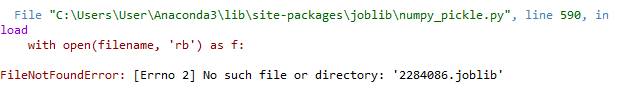
\includegraphics[scale=0.8]{figures/error1.PNG}
    \end{figure}
    \begin{figure}[!htbp]
    \centering
    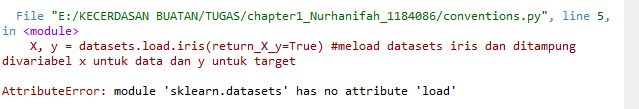
\includegraphics[scale=0.8]{figures/error2.PNG}
    \end{figure}
\item Tuliskan kode error dan jenis error
\par 
FileNotFoundError ( file tidak ditemukan pada saat kita menjalankan program).\\
AttribututeError
\item Solusi dari error tersebut
\par 
pertama yaitu salah dalam penulisan filenya kemudian typo pada penulisan codenya. jadi kita dalam membuat code harus lebih teliti lagi.
\end{enumerate}


